\subsection{Neuro-formal verification: the whole picture}
\label{sec:northstar}

\paragraph{The inputs.} A developer has a program $P_L$ in some source language
$L$; a property $S_{nl}$ they care about, written in whatever notation they
already use --- a docstring, an issue, a comment; and an environment $E$ in
which the program executes --- including the context that calls it and the
libraries and services it calls --- described by documentation $E_{nl}$.

\paragraph{The workflow.} Figure~\ref{fig:northstar} lays out five stages that
turn those inputs into a checked proof over a model of a program and return it
in the developer's own terms.
The workflow is parameterized by a verification-aware language $F$ with
first-class formal verification support.

\begin{enumerate}
\item \textbf{Intent formalization}~\cite{lahiri2026intent}.
  Synthesize from $E_{nl}$ a formal specification $E_F$ in $F$ --- the
  contracts of the libraries the program calls and any preconditions stated
  by the documentation --- and from $S_{nl}$ an assertion $S_L$ in the source
  language that expresses what the developer meant. Both are claims about intent, and
  both should be \emph{attested} against every artifact available --- the
  documentation, the tests, and the source when available.
\item \textbf{Program translation}, $P_L \rightarrow P_F$, into the formal
  language $F$ of some mature verifier. This step can 
  range from purely symbolic (a compiler, where a faithful front end exists)
  through mixed approaches to purely neural (this paper).
\item \textbf{Specification translation}, $S_L \rightarrow S_F$, along the same
  spectrum.
\item \textbf{Proof search over $F$}, discharged by the verifier for $F$ and
  driven agentically: an agent proposes invariants, lemmas, and tactics; the
  verifier checks each proposal, so the search may use neural methods freely
  without putting the verifier's soundness at risk.
\item \textbf{Proof mapping.} Map a successful formal proof
  $\mathit{Proof}(P_F, S_F, E_F)$ into a \emph{proof sketch} stated over $P_L$,
  using the developer's own variables and naming the assumptions in terms of
  $E_{nl}$.
\end{enumerate}

The workflow should not be construed as end-to-end formal verification that
$P_L$ satisfies $S_L$. The
source-language semantics, the environment description, and the translations
are not all formally attested. We therefore use the term \emph{formal program
reasoning}.

\paragraph{Proof beyond the final verdict.} Formal proof is not confined to
establishing $S_F$ for $P_F$ under $E_F$. Intent formalization can also produce
a test suite $T_F$, either extracted from library artifacts or generated by
agents, together with proofs of the soundness, completeness, and preciseness of
$E_F$ with respect to $T_F$~\cite{lahiri2026intent}. Similarly, the path from
$S_{nl}$ to $S_F$ can produce tests and proofs attesting $S_F$. These artifacts
strengthen the attestation of the formalized environment and specification,
even though they do not establish end-to-end correctness.
More generally, the explicit formal artifacts $P_F$, $S_F$, and $E_F$ give
users inspectable accounts of the program model, the property being checked,
and the assumptions under which the result holds. A user can review these
artifacts, identify mismodeling, and provide feedback that improves subsequent
formalization.
Users can also vet familiar concrete tests rather than inspect $S_F$ and $E_F$
directly, reducing the formal-methods expertise required of them.

\begin{figure}[t]
\centering
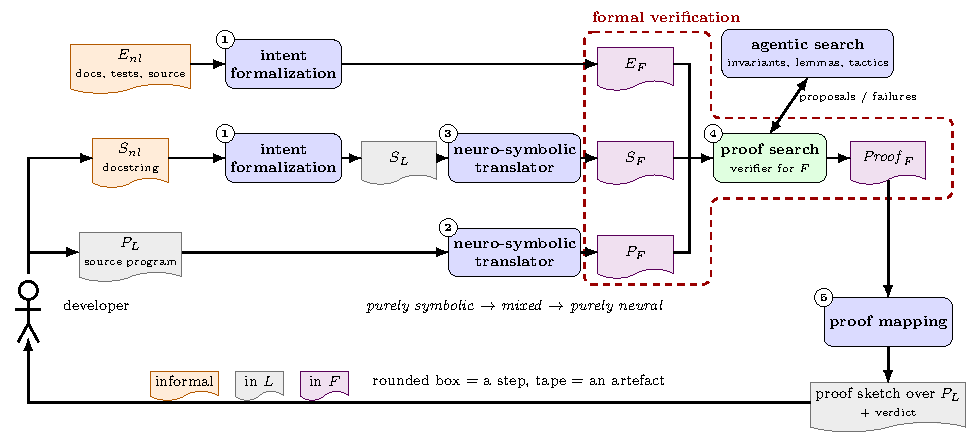
\includegraphics[width=\linewidth]{figs/northstar}
\caption{Neuro-formal verification. Circled numbers are the five stages
enumerated above. Rounded boxes transform; tape-shaped nodes are the
artifacts they consume and produce, colored by the language the artifact lives
in --- orange for informal English, gray for the source language $L$, purple for
the formal language $F$. Blue is a step an LLM performs, green a step a verifier
performs. The developer authors $S_{nl}$ and $P_L$ and reads the proof
sketch that comes back. The dashed red region is the classical formal
verification problem --- given $P_F$, $S_F$ and $E_F$, find a proof.}
\label{fig:northstar}
\end{figure}

\subsection{An example}
\label{sec:example}

Let us illustrate the workflow for this paper with a simple two-line Python program.
We restrict the list elements to be exact rationals
(Python's \texttt{fractions.Fraction}), so that the division operator \texttt{/} performs no rounding ---
an assumption needed for the specification to hold.

\begin{center}
\begin{minipage}{0.74\linewidth}
\begin{lstlisting}[language=Python,basicstyle=\ttfamily\footnotesize,columns=fullflexible,keepspaces=true]
def shifted_mean(l):
    "Average the list after adding 1 to each element; l must be non-empty."
    return sum(x + 1 for x in l) / len(l)

# postcondition
assert shifted_mean(l) == sum(l) / len(l) + 1
\end{lstlisting}
\end{minipage}
\end{center}

\noindent
Informally, the correctness of this specification relies on
 \[
  \mathit{len}(l) \neq 0
 \] 
and 
\[
  \mathit{sum}(\,\{x+1 \mid x \in l\}\,) \;=\; \mathit{sum}(l) + \mathit{len}(l).
\]

Stage~5 would not only return ``verified'' but also the proof-sketch reasoning, in natural language: \emph{the specification
holds because adding $1$ to each of \texttt{len(l)} elements adds
\texttt{len(l)} to their sum, provided the list is non-empty} --- an artifact the developer can check.

\paragraph{The same example, worked in \daf{}.} Instantiating $F$ with \daf{}
makes the workflow concrete. Stage~1 starts from $E_{nl}$, which for
this program is the documentation of Python's \texttt{sum}\footnote{The
built-in's runtime docstring --- \texttt{sum.\_\_doc\_\_} in CPython~3.14 --- quoted
as it stands, less a closing sentence restricting it to numeric values.} --- all that is
actually on offer about the library:

\begin{center}
\begin{minipage}{\linewidth}
\begin{lstlisting}[basicstyle=\ttfamily\normalsize,columns=fullflexible,keepspaces=true,frame=none]
Return the sum of a 'start' value (default: 0) plus an iterable of numbers.
When the iterable is empty, return the start value.
\end{lstlisting}
\end{minipage}
\end{center}

\noindent
Stage~1 formalizes this documentation as $E_F$, which in this example consists
only of a recursive definition of \texttt{Sum}:

\begin{center}
\begin{minipage}{0.86\linewidth}
\begin{lstlisting}[language=Dafny,basicstyle=\ttfamily\footnotesize,columns=fullflexible,keepspaces=true]
function Sum(l: seq<real>): real {
  if |l| == 0 then 0.0 else l[0] + Sum(l[1..]) }
\end{lstlisting}
\end{minipage}
\end{center}

\noindent
\texttt{Sum} is attestable against the docstring: it is a recursive definition
whose base and recursive cases can be read directly against the documented
behavior.

Stages~2 and~3 then render $P_F$ and $S_F$. Translating the generator expression
\texttt{x + 1 for x in l} introduces \texttt{Shift} as part of the model of
$P_F$; it is not part of $E_F$:

\begin{center}
\begin{minipage}{0.86\linewidth}
\begin{lstlisting}[language=Dafny,basicstyle=\ttfamily\footnotesize,columns=fullflexible,keepspaces=true]
function Shift(l: seq<real>): seq<real> {
  seq(|l|, i requires 0 <= i < |l| => l[i] + 1.0) }

method ShiftedMean(l: seq<real>) returns (r: real)
  requires |l| > 0
  ensures r == Sum(l) / (|l| as real) + 1.0
{ ShiftedSum(l);
  var n := |l| as real;
  r := Sum(Shift(l)) / n;
  DivDistrib(Sum(l), n); }
\end{lstlisting}
\end{minipage}
\end{center}

\noindent
The two calls in the method are proof steps, not part of $P_F$. Stage~4
introduces both lemmas. \texttt{ShiftedSum} proves by induction that translating
the generator preserves the expected relationship between the two sums.
\texttt{DivDistrib} supplies the nonlinear arithmetic step that the verifier
does not close automatically when $n$ is symbolic:

\begin{center}
\begin{minipage}{0.86\linewidth}
\begin{lstlisting}[language=Dafny,basicstyle=\ttfamily\footnotesize,columns=fullflexible,keepspaces=true]
lemma ShiftedSum(l: seq<real>)
  ensures Sum(Shift(l)) == Sum(l) + |l| as real
{ if |l| > 0 {
    assert Shift(l)[1..] == Shift(l[1..]);
    ShiftedSum(l[1..]); } }

lemma DivDistrib(a: real, n: real)
  requires n != 0.0
  ensures (a + n) / n == a / n + 1.0
{ assert n / n == 1.0;
  assert (a + n) / n == a / n + n / n; }
\end{lstlisting}
\end{minipage}
\end{center}

\noindent
\daf{} checks both lemmas and, with their calls in
\texttt{ShiftedMean}, discharges all seven obligations of the resulting file.
Stage~5 would map this proof back to the proof-sketch reasoning stated above:
\emph{the specification holds because adding $1$ to each of \texttt{len(l)}
elements adds \texttt{len(l)} to their sum, provided the list is non-empty}.
The current instantiation evaluated in this paper does not include this mapping.


\paragraph{The same example with a bug, refuted.} 
Suppose the
developer had written the reduction as a single addition on the total rather
than one per element --- \texttt{r := (Sum(l) + 1.0) / n} in place of
\texttt{r := Sum(Shift(l)) / n}, a one-token slip.

\begin{center}
\begin{minipage}{0.74\linewidth}
\begin{lstlisting}[language=Python,basicstyle=\ttfamily\footnotesize,columns=fullflexible,keepspaces=true]
def shifted_mean(l):
    "Average the list after adding 1 to each element; l must be non-empty."
    return (sum(l) + 1) / len(l)  # bug
\end{lstlisting}
\end{minipage}
\end{center}

\noindent
Now $P_F$ does not meet
$S_F$, and stage~5 should say so. The tempting move is to report the verifier's
failure: \daf{} cannot prove the postcondition.
However, a proof failure cannot be interpreted as a bug --- an unproved goal is evidence about
the proof search, not about the program.

What makes a refutation attestable is the same thing that makes a verification
attestable --- a proof that $S_F$ fails. The program is left untouched, $S_F$ is
negated, and the witness is added as a precondition, so the verifier is asked to
confirm a positive claim rather than to fail at a negative one:

\begin{center}
\begin{minipage}{0.86\linewidth}
\begin{lstlisting}[language=Dafny,basicstyle=\ttfamily\footnotesize,columns=fullflexible,keepspaces=true]
method ShiftedMean(l: seq<real>) returns (r: real)
  requires |l| > 0
  requires l == [0.0, 0.0]                      // the witness
  ensures !(r == Sum(l) / (|l| as real) + 1.0)  // S_F, negated
{ var n := |l| as real;
  r := (Sum(l) + 1.0) / n;                      // the bug
  assert Sum(l) == l[0] + Sum(l[1..]);
  assert Sum(l[1..]) == l[1] + Sum(l[1..][1..]);
  assert l[1..][1..] == []; }
\end{lstlisting}
\end{minipage}
\end{center}

\noindent
The witness $l = [0,0]$ makes the buggy program return $1/2$ where
$S_F$ demands $1$; the three asserts are the proof-repair loop unfolding
\texttt{Sum} on that input, and \daf{} discharges the negated goal. 
On the Python list \texttt{[Fraction(0), Fraction(0)]} the buggy program itself returns
\texttt{Fraction(1, 2)} where the specification demands \texttt{Fraction(1)}, and the
\texttt{assert} raises \texttt{AssertionError}. 
